\graphicspath{{content/chapters/5_design/figures/}}
\chapter{Design}
\label{chp:design}

This chapter outlines the core design components that form the foundation of the speech enhancement system. It begins by addressing the challenge of handling variable length audio inputs, essential for batch-based model training. The latter and more substantial section focuses on the design of the \gls{ml} architectures used in this project. Detailing each model's structure and the reasoning behind their implementation for speech enhancement.

\section{Variable Length Handling}
\label{sec:variable_length_handling}

For this project, only the clean and noisy pairs of audio files from the dataset are required. The transcript text files are ignored, as they are not relevant to the task. However, such transcripts are valuable in tasks like speech recognition or text-to-speech. As highlighted in the dataset analysis in Section~\ref{sec:dataset_exploration}, the audio files vary in length. This poses a challenge for model training, as batch processing requires input tensors to have consistent dimensions.

To address this, several algorithms for handling variable-length audio inputs were explored. The most basic approach involves padding each audio file to match the length of the longest sample in the batch, typically by appending zeros to the end of shorter files. While this method is simple, it has significant drawbacks. Excessive padding introduces unnecessary data that may act as noise during training, making it harder for the model to learn effectively. The greater the variation in input lengths, the more padding is required, which can negatively impact overall training performance.

\begin{figure}[h]
    \centering
    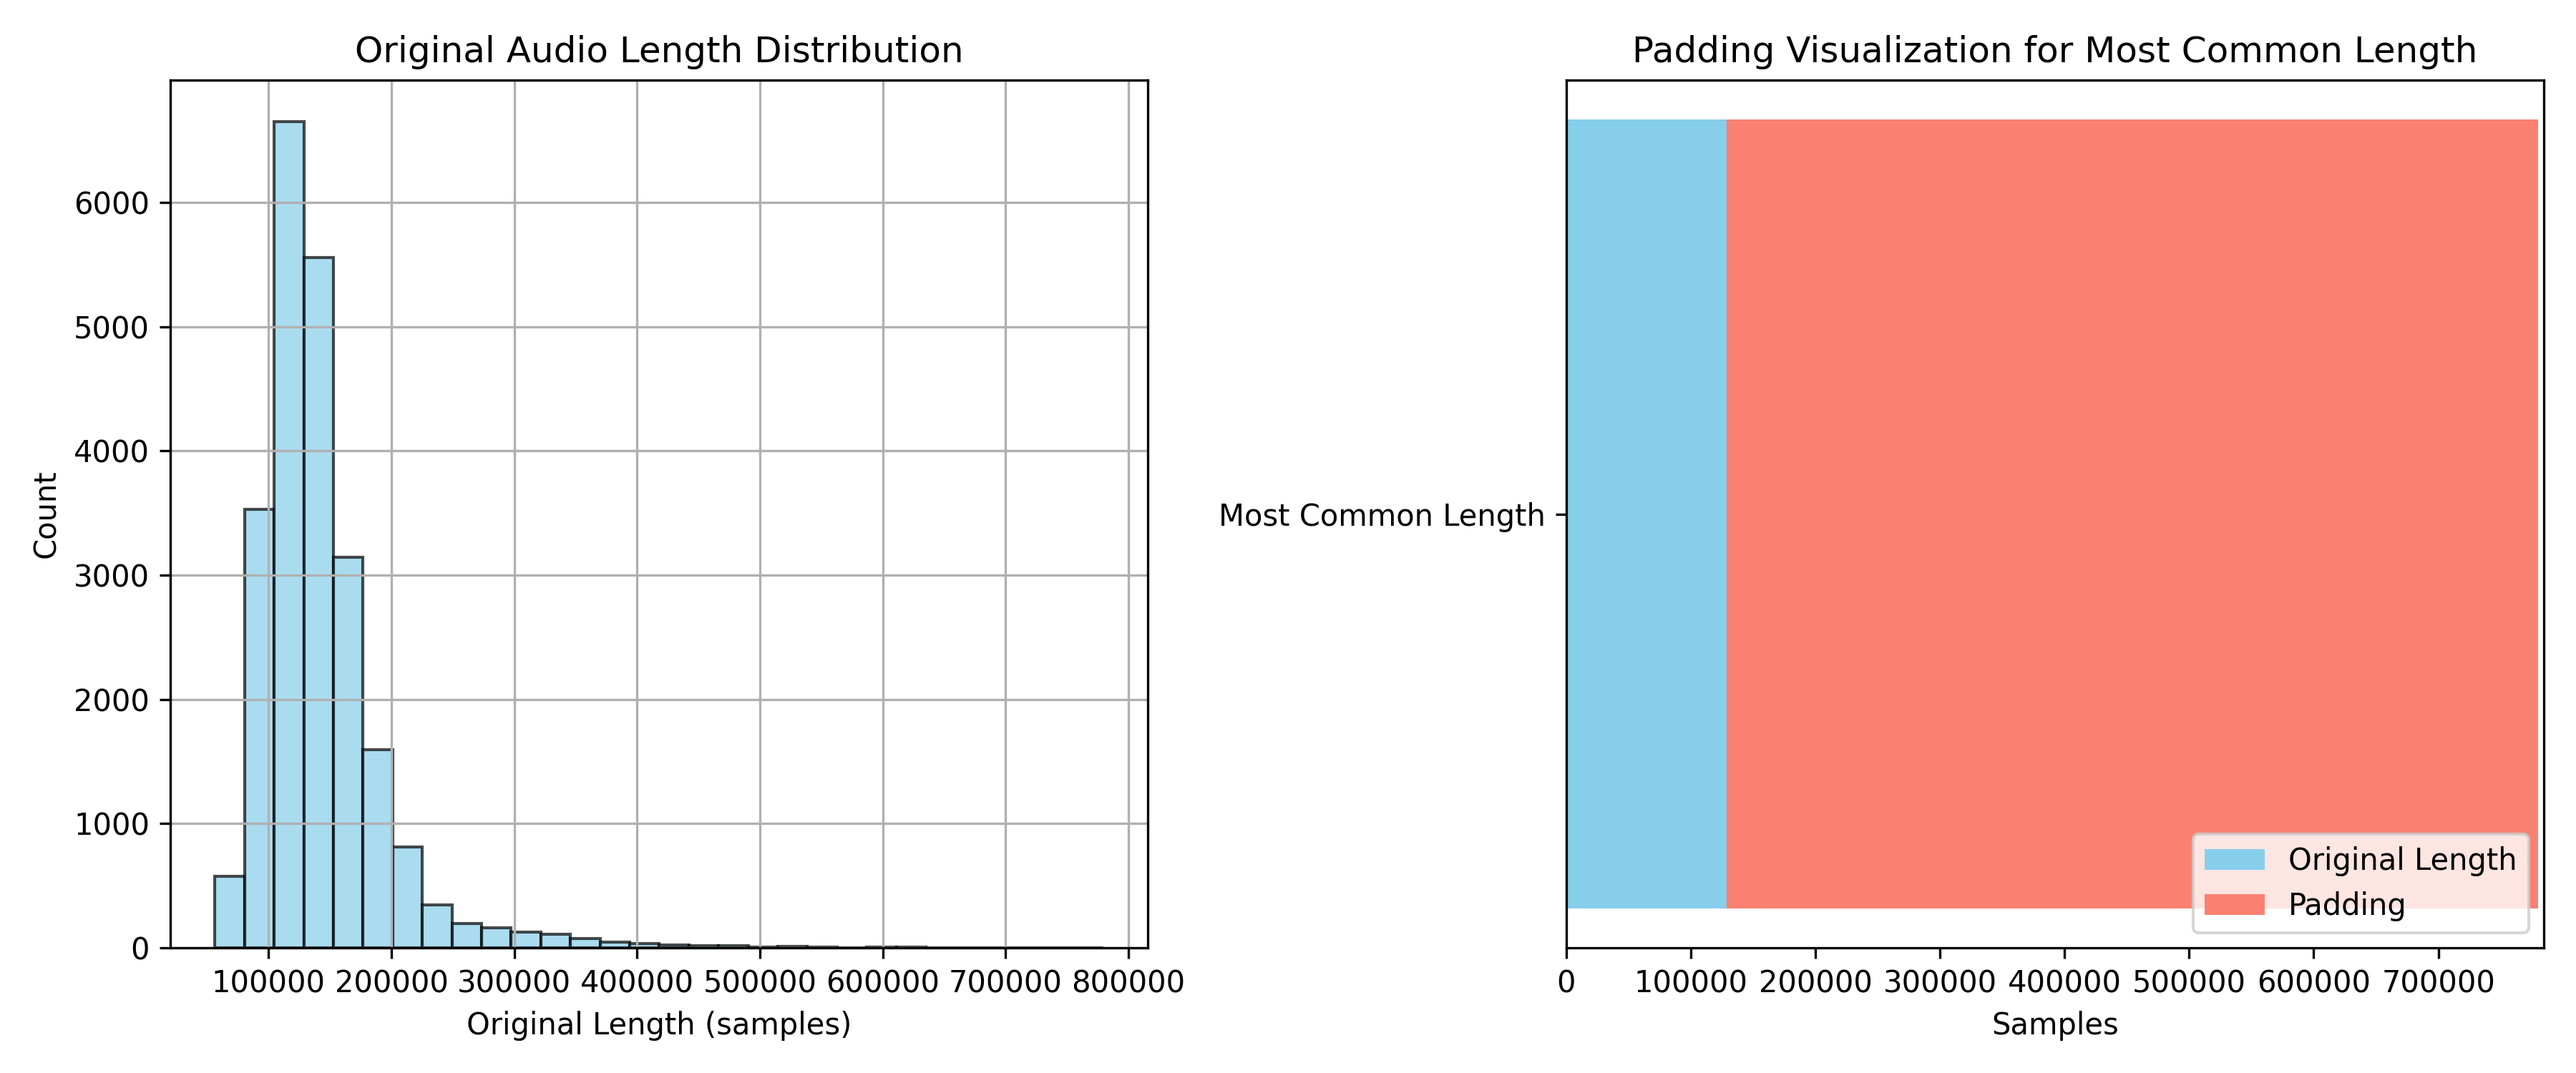
\includegraphics[width=\textwidth,keepaspectratio]{max_padding.png}
    \caption{\label{fig:max_padding}Illustration of maximum-length padding.}
\end{figure}

As shown in Figure~\ref{fig:max_padding}, the most common audio length is padded so heavily that the padding exceeds the actual content. This is far from ideal. To mitigate this issue, three different padding strategies were used, each aimed at reducing excessive padding.

The first method is \textit{Static Bucketing}, which groups audio files into predefined fixed-length buckets, reducing the amount of unnecessary padding. The second method, \textit{Dynamic Bucketing}, builds on this by creating buckets dynamically based on the distribution of audio lengths, offering a more adaptive grouping approach. The third and final method, introduced in Section~\ref{sec:distortion_free_handling}, is the \gls{pto}. A more sophisticated approach that combines padding and truncating to minimise distortion in the data.

All three methods were implemented for testing and evaluation. Their role in the system design is critical, as they help ensure that the model can learn effectively without being hindered by dimensional mismatches or excessive zero-padding. Further details on their implementations are provided in Chapter~\ref{chp:implementation}, and their impact on model performance is discussed in Chapter~\ref{chp:evaluation}.

\section{Model Architecture}
\label{sec:model_architecture}

The model architecture is central to system design, defining how inputs are processed, features transformed, and outputs reconstructed. The project’s modular structure supports exploring various neural networks, starting from a simple baseline and extending to more advanced models. As introduced in Section~\ref{sec:autoencoders}, all models follow the autoencoder paradigm and operate on spectrograms, with real and imaginary components concatenated into a two-channel input and producing a similar two-channel output.

Initially, a \texttt{Tanh} activation was used at the output layer to constrain values within $[-1, 1]$, aiming for numerical stability during inverse \gls{stft}. However, evaluations showed this suppressed amplitude dynamics and degraded denoising performance. The \texttt{Tanh} was therefore removed from all model outputs—an improvement detailed in Appendix~\ref{appendix:tanh_removal}.

\subsection{Convolutional Neural Network}
\label{sec:cnn}

The \gls{cnn} model implemented in this project serves as the baseline architecture. Its design follows a widely used encoder-decoder structure, commonly found in literature. A corresponding visual representation of the implemented architecture was created in Figure~\ref{fig:cnn}. The model operates on concatenated real and imaginary spectrogram components, processed as a two-channel input. Its straightforward structure makes it suitable for benchmarking and for validating the core pipeline before exploring more advanced architectures.

The first entry point in the forward pass of the model is the encoder. The encoder consists of three convolutional layers, each followed by a \gls{prelu} activation function. Each convolution uses a \(3 \times 3\) kernel. The network begins with 2 input channels and progressively increases to 128 channels. The encoder's role is to reduce the spatial dimensions of the input while increasing the number of feature channels.

\begin{figure}[h]
    \centering
    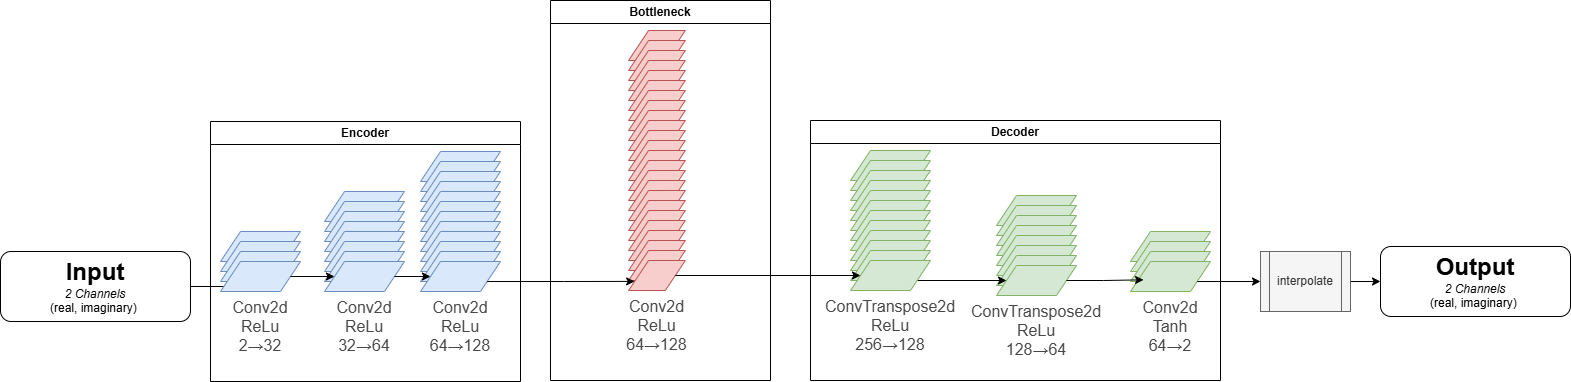
\includegraphics[width=\textwidth,keepaspectratio]{cnn.png}
    \caption{\label{fig:cnn}Basic CNN architecture.}
\end{figure}

The output of the encoder is passed to a bottleneck layer, which further transforms the feature space without altering its spatial resolution. In this implementation, the bottleneck consists of a single \(3 \times 3\) convolutional layer that increases the number of channels from 128 to 256, followed by a \gls{relu} activation. This design deepens the network and allows for more complex feature extraction. Since the bottleneck is not part of the downsampling or upsampling path, it also encourages the decoder to learn a more challenging mapping from latent space back to the input resolution.

The decoder reconstructs the spectrogram from the transformed features using a three-stage transposed convolutional block. It includes two transposed convolutional layers that upsample the spatial dimensions, reversing the compression performed by the encoder. Each is followed by a \gls{relu} activation. A final standard \(3 \times 3\) convolutional layer reduces the channel count from 64 to 2, corresponding to the real and imaginary parts of the output spectrogram. To ensure output consistency, bilinear interpolation is applied to match the original input resolution prior to splitting the output into its two channels.

While simple, this model plays a critical role in establishing a baseline performance level. It validates system functionality and serves as a reference for later architectures. The \gls{cnn} model is straightforward to implement and interpret, making it a suitable starting point for benchmarking and guiding the development of more sophisticated architectures introduced in subsequent sections.

\subsection{Convolutional Encoder Decoder}
\label{sec:ced}

The \gls{ced} architecture implemented in this project is based on the design proposed by Park and Lee~\cite{park2017acoustic}, as reviewed in Section~\ref{sec:fcns}. The model follows a symmetric encoder-decoder structure, operating on complex spectrograms represented as two-channel inputs (real and imaginary concatenated along the channel dimension).

The encoder is composed of five convolutional blocks. Each block consists of a convolutional layer with a tall vertical kernel, batch normalisation, a \gls{relu} activation function, and a \(2 \times 1\) max pooling operation. The vertical kernel sizes decrease from \(13 \times 1\) to \(5 \times 1\) across layers, preserving frequency resolution while downsampling the temporal dimension. The number of channels increases progressively from 2 to 32, enabling richer feature representations as the input is compressed.

\begin{figure}[h]
    \centering
    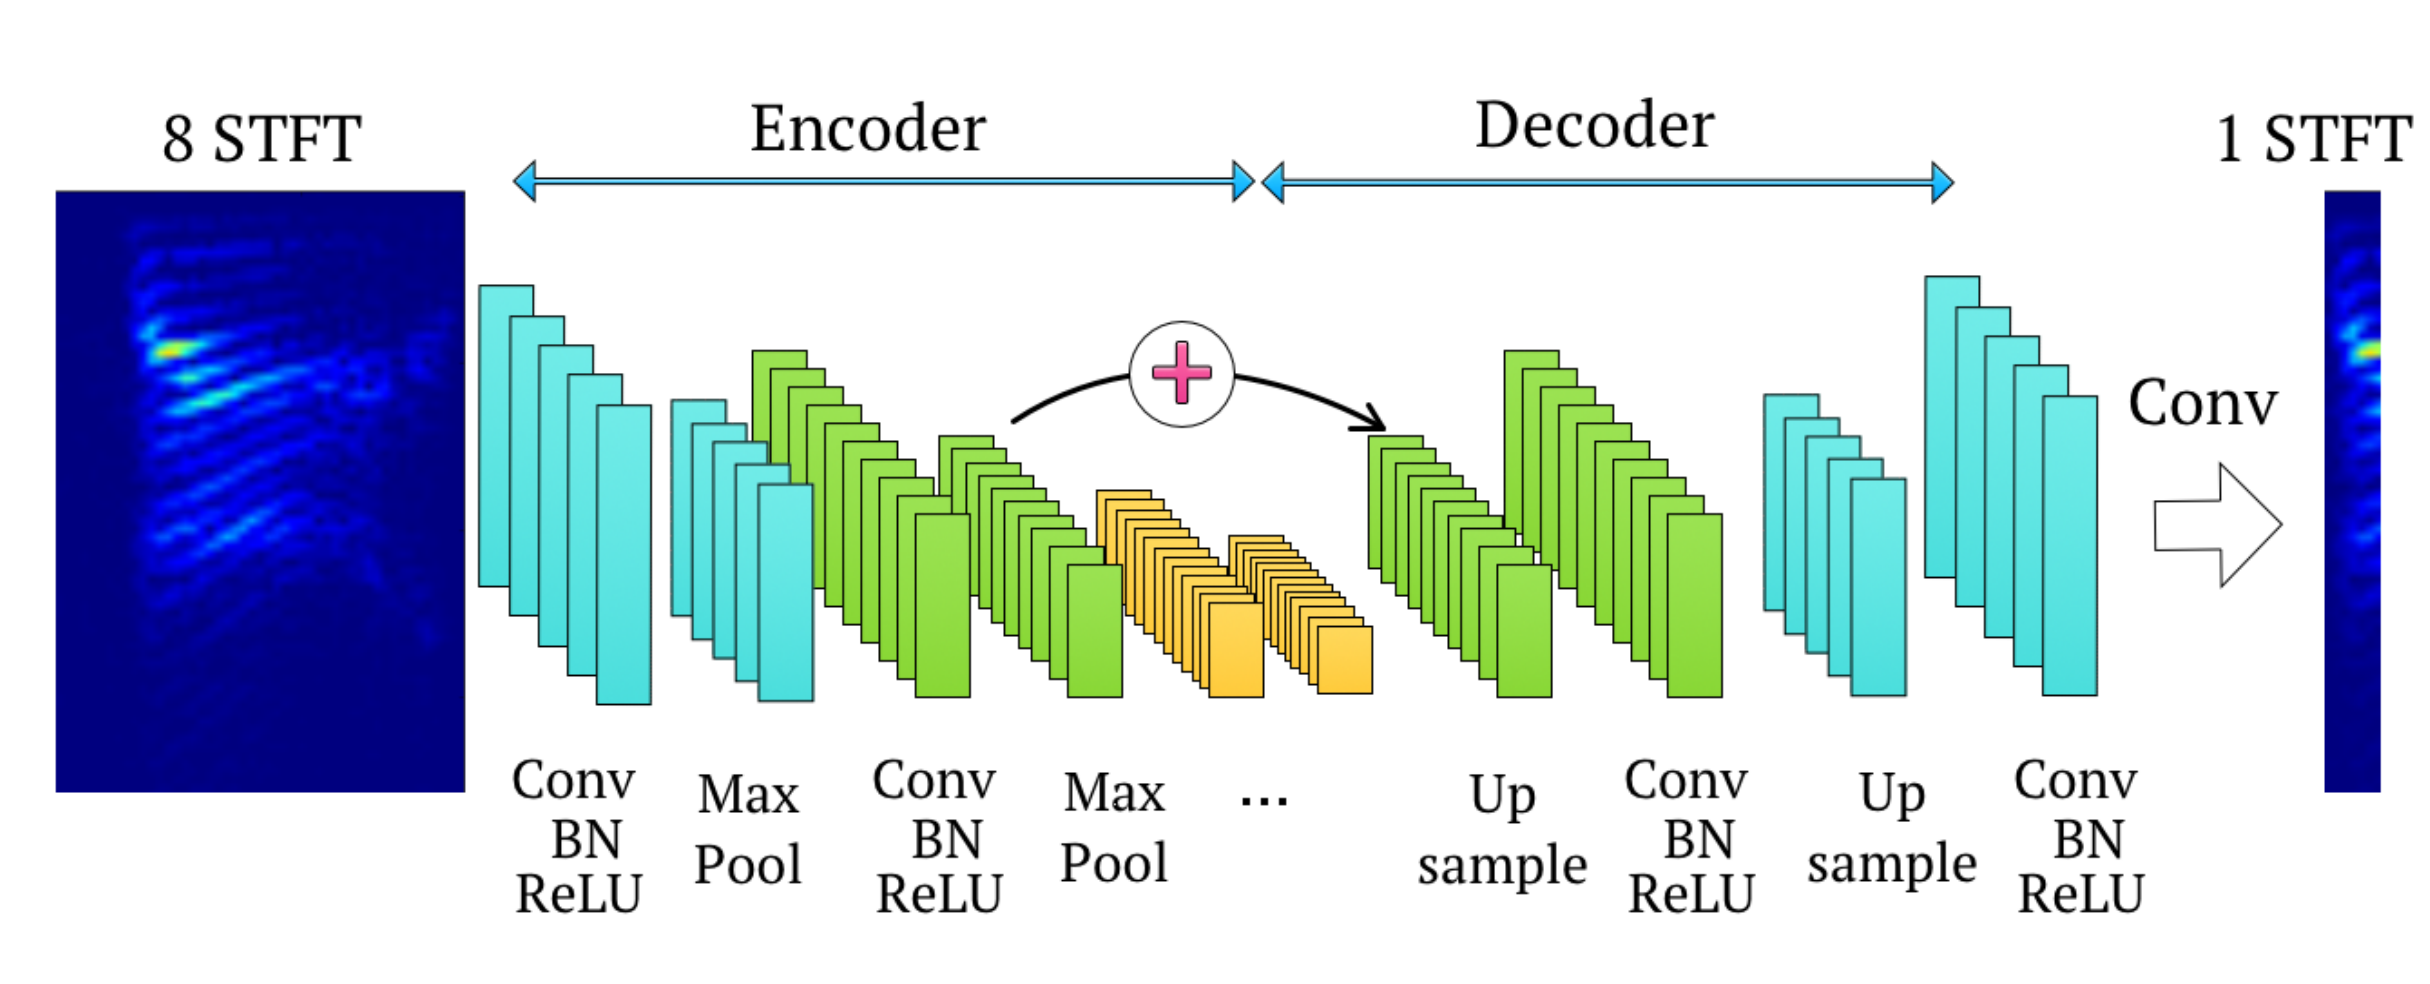
\includegraphics[width=\textwidth,keepaspectratio]{ced.png}
    \caption{\label{fig:ced}CED Network \cite{park2017acoustic}.}
\end{figure}

Unlike the \gls{cnn} baseline, which uses a dedicated bottleneck for feature transformation, the \gls{ced} model omits this step. Its encoder and decoder are seen to be fully connected in Figure~\ref{fig:ced}. They are connected through a continuous intermediate representation, avoiding abrupt compression. This enables smoother feature transitions across the network. Beneficial for speech signals where such disruptions can degrade temporal patterns.

The decoder mirrors the encoder in structure, using four stages of upsampling followed by convolution, batch normalisation, and \gls{relu} activation. Each upsampling layer doubles the temporal dimension using a scale factor of \((2, 1)\), restoring the resolution reduced in the encoder. The decoder reverses the channel progression, reducing from 32 back down to 12. A final convolutional layer with a large vertical kernel of \(129 \times 1\) is used to project the output to two channels, corresponding to the real and imaginary parts of the denoised spectrogram. A bilinear interpolation step is applied at the end to ensure the output matches the original input resolution.

By eliminating the bottleneck and employing deep, temporally aware convolutional transformations, the \gls{ced} model enables a smooth and information preserving mapping from noisy to clean spectrograms. Its symmetric structure, combined with frequency preserving vertical kernels and temporal downsampling, makes it well suited for capturing sequential dependencies without sacrificing spectral resolution. In this project, the \gls{ced} architecture is used as a strong benchmark for assessing the effectiveness of \gls{fcn} encoder-decoder, particularly in contrast to the more compressed representations used in \gls{cnn}-based designs.

\subsection{Redundant Convolutional Encoder Decoder}
\label{sec:rced}

The \gls{rced} architecture implemented in this project builds upon the \gls{ced} framework introduced by Park and Lee~\cite{park2017acoustic} and discussed in Section~\ref{sec:fcns}. Like the \gls{ced}, \gls{rced} operates on complex spectrograms represented as two-channel inputs (real and imaginary). However, the design omits all pooling and upsampling operations to preserve full temporal and spectral resolution throughout the network. This is shown in the architecture diagram sampled from the original paper in Figure~\ref{fig:rced}.

\begin{figure}[h]
    \centering
    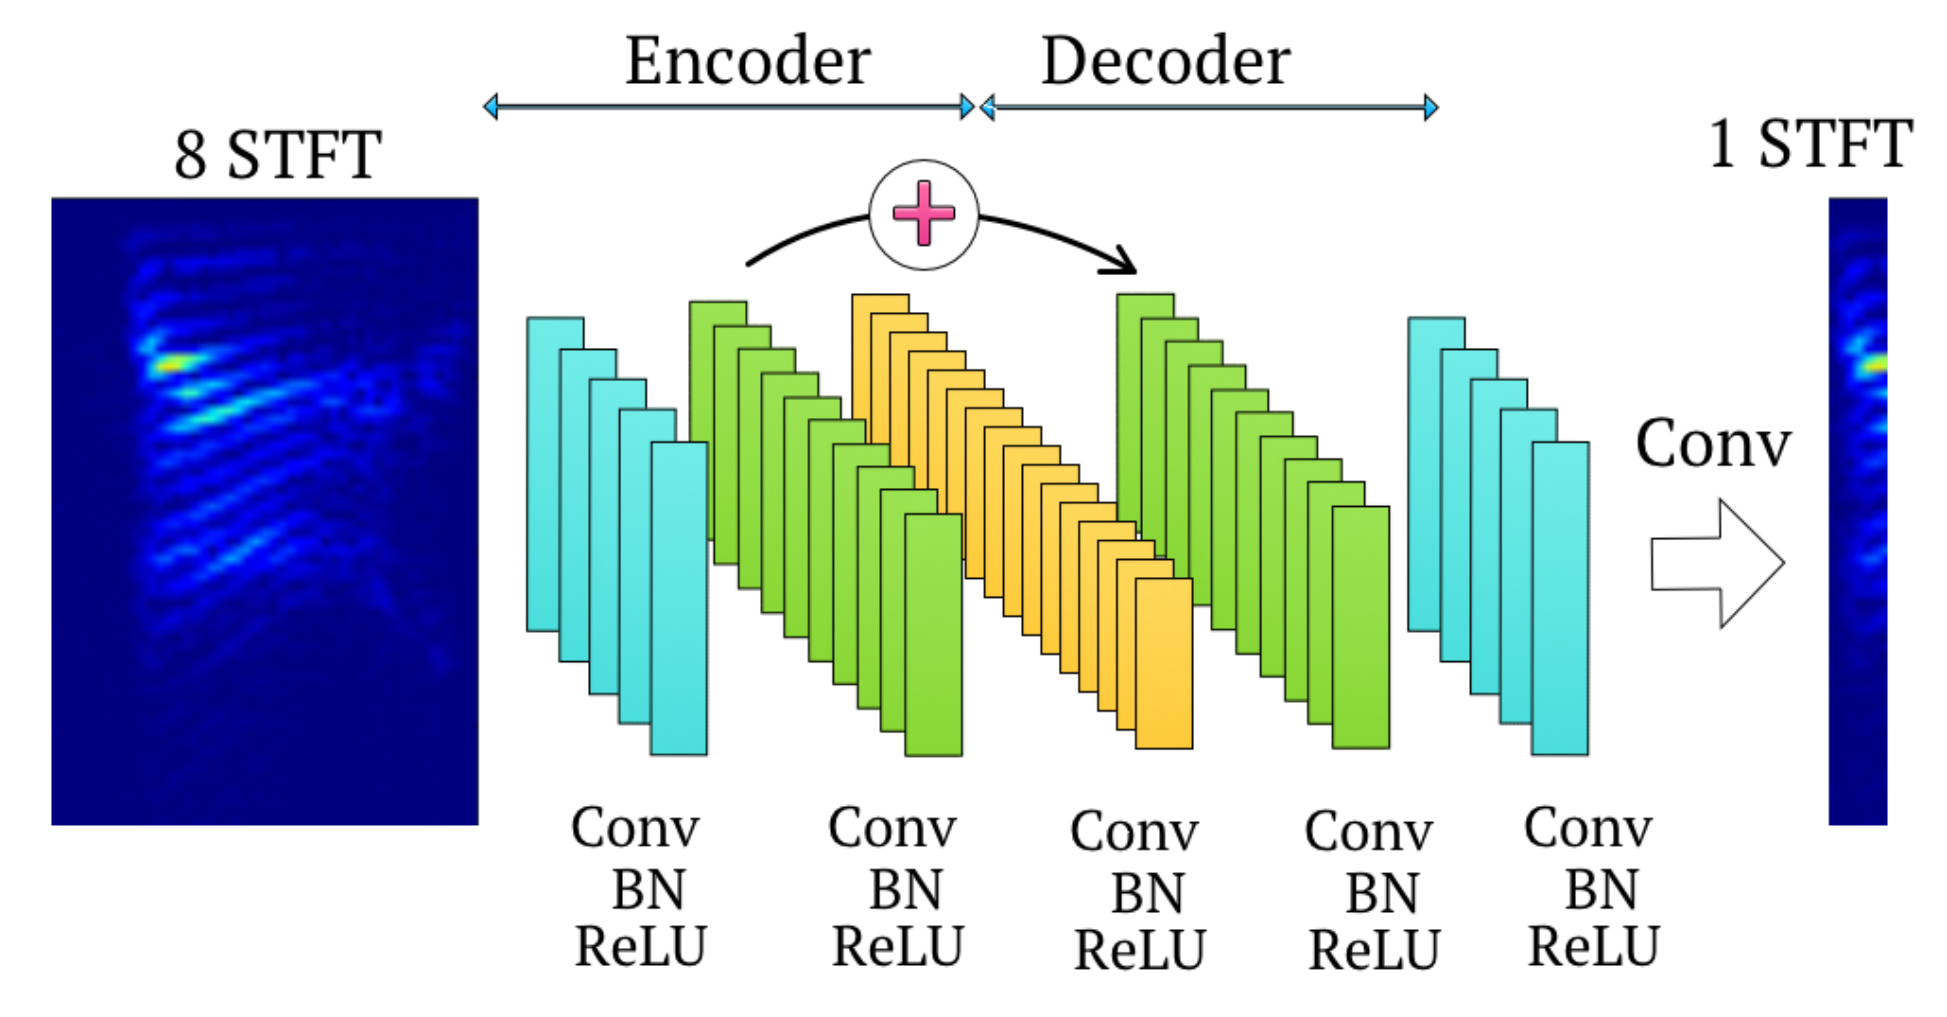
\includegraphics[width=\textwidth,keepaspectratio]{r-ced.png}
    \caption{\label{fig:rced}RCED architecture \cite{park2017acoustic}.}
\end{figure}

The network is composed of nine sequential convolutional layers. The first eight layers use tall vertical kernels ranging from \(13 \times 1\) to \(7 \times 1\), symmetrically arranged around the network's midpoint. Each layer is followed by a \gls{relu} activation and batch normalisation. The number of channels increases from 2 to 32 in the first half and then mirrors back to 12 in the second half, following the filter progression: 12, 16, 20, 24, 32, 24, 20, 16, 12. This symmetric arrangement enables the model to gradually build and refine feature representations without disrupting the resolution of the input signal.

Unlike typical encoder-decoder models, the \gls{ced} maintains a constant spatial resolution throughout the network. Instead of using pooling or upsampling layers, it increases representational depth by stacking additional convolutional layers. This improves expressiveness while preserving time-frequency alignment, which is essential for speech enhancement. A final 
\(129 \times 1\) convolution projects the output to two channels (real and imaginary), followed by bilinear interpolation to restore the original resolution.

By eliminating dimensionality altering operations and relying on a deeper sequence of convolutional blocks, the \gls{ced} model is able to maintain high resolution feature representations across all layers. This architecture is especially useful in applications where preserving the fine structure of spectrograms is essential. In this project, \gls{ced} is evaluated as a resolution preserving alternative to encoder-decoder architectures.

\subsection{U-Net}
\label{sec:unet}

The \gls{unet} model implemented in this project is adapted from the widely known \gls{unet} architecture originally proposed for biomedical image segmentation~\cite{ronneberger2015unet}.In this work, the architecture is repurposed for speech enhancement using complex spectrograms. A corresponding diagram was constructed to illustrate the adaptation (Figure~\ref{fig:unet}). The model follows a symmetric encoder-decoder structure with skip connections and is designed to recover clean speech signals by operating directly on the concatenated real and imaginary spectrogram components.

The encoder consists of five convolutional blocks, each followed by instance normalisation and a \gls{prelu} activation. Downsampling is achieved by using a stride of 2 in all but the first convolution block. The channel depth increases progressively from 2 to 1024 across the five stages: \(2 \rightarrow 64 \rightarrow 128 \rightarrow 256 \rightarrow 512 \rightarrow 1024\). Instance normalisation is preferred over batch normalisation for improved stability with variable-length or low-batch-size audio inputs.

\begin{figure}[h]
    \centering
    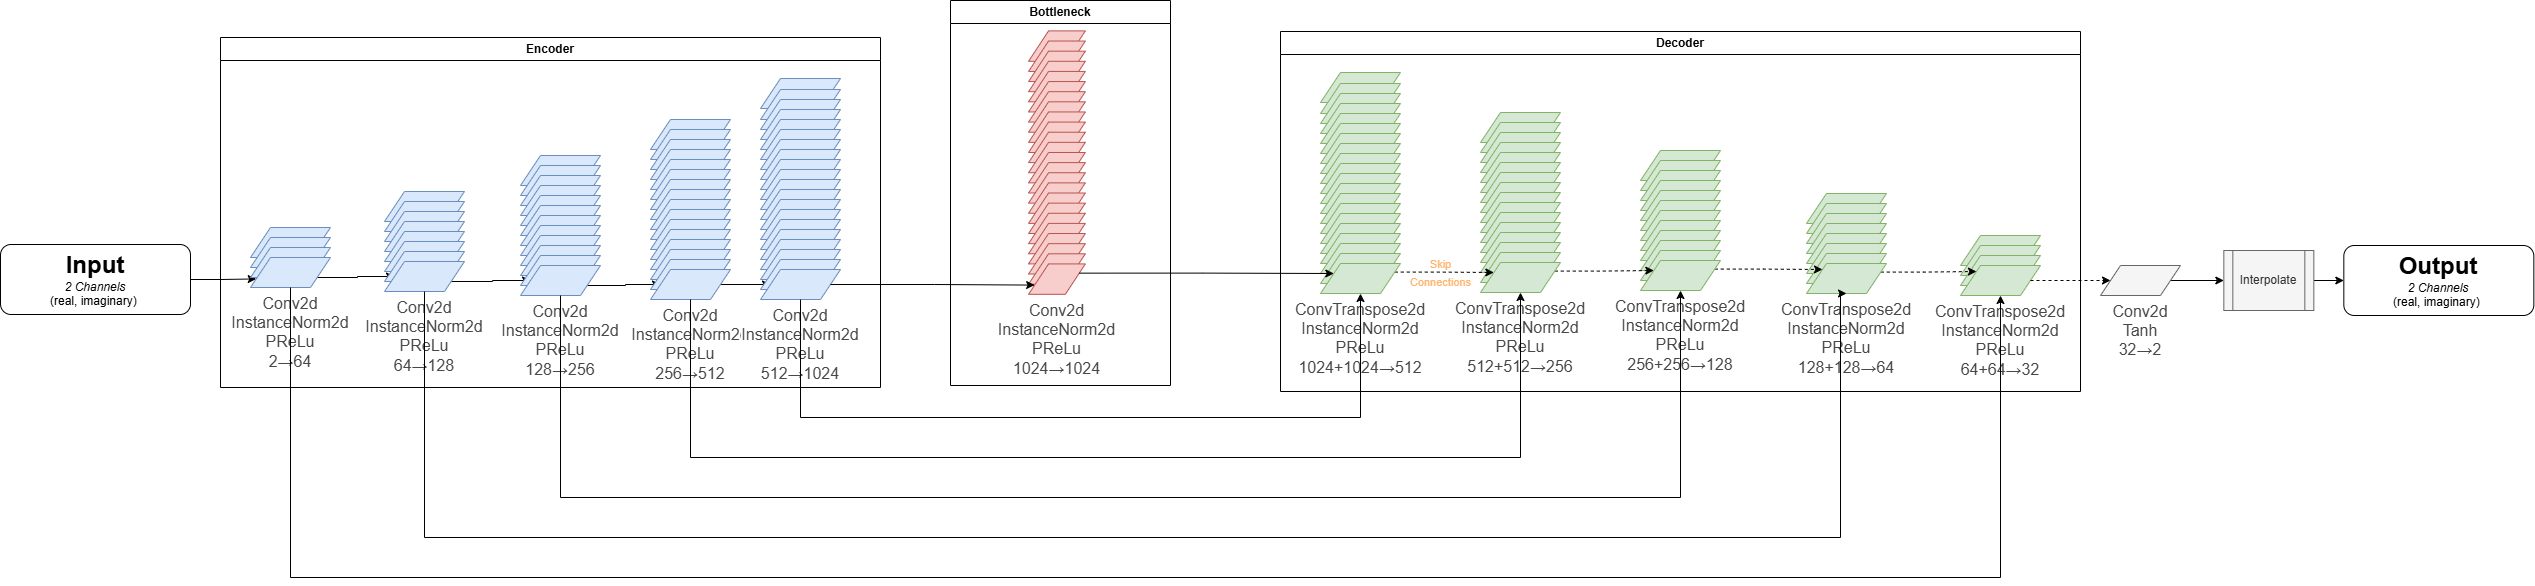
\includegraphics[width=\textwidth]{unet.png}
    \caption{\label{fig:unet}UNet Architecture.}
\end{figure}

At the centre of the network is a bottleneck block that maintains the 1024-channel depth while applying an additional convolution, instance normalisation, and \gls{prelu} activation. Unlike traditional bottlenecks that compress the latent representation, this layer serves as a non-linear transformation hub that enhances the feature space before decoding.

The decoder mirrors the encoder with five transposed convolutional blocks that upsample feature maps and reduce channel depth through the sequence \(1024 \rightarrow 512 \rightarrow 256 \rightarrow 128 \rightarrow 64 \rightarrow 32\). At each stage, features from the corresponding encoder block are concatenated with the upsampled output via skip connections. Since downsampling alters spatial resolution, bilinear interpolation is applied to align encoder features before concatenation and again after the final \(3 \times 3\) convolution, which projects the output to 2 channels corresponding to the real and imaginary components of the denoised spectrogram.

This \gls{unet} implementation preserves the architectural strengths of the original model while tailoring its structure for speech enhancement. The use of skip connections, instance normalisation, and a deep encoder-decoder hierarchy enhances the model’s ability to recover spectrogram-temporal structure, making it a powerful architecture for complex denoising tasks.

\subsection{Conv-TasNet}
\label{sec:convtasnet}

The \gls{convtasnet} model implemented in this project is based on the architecture proposed by Luo and Mesgarani~\cite{Luo2018ConvTasNetSI}, as discussed in Section~\ref{sec:convtasnet_lit_review}. A corresponding architecture diagram, shown in Figure~\ref{fig:convtasnet}, is sourced from the original paper. Although the core structure is preserved, several adaptations were made to align the model with the spectrogram-based input framework used throughout this system.

The original \gls{convtasnet} operates directly on time-domain audio signals. In contrast, this implementation modifies the input format to handle complex-valued spectrograms. The real and imaginary components are concatenated along the channel dimension, forming a two-channel input that is passed through a \(3 \times 3\) convolutional encoder. The encoder projects the input to 128 channels using dynamic padding to preserve resolution.

\begin{figure}[h]
    \centering
    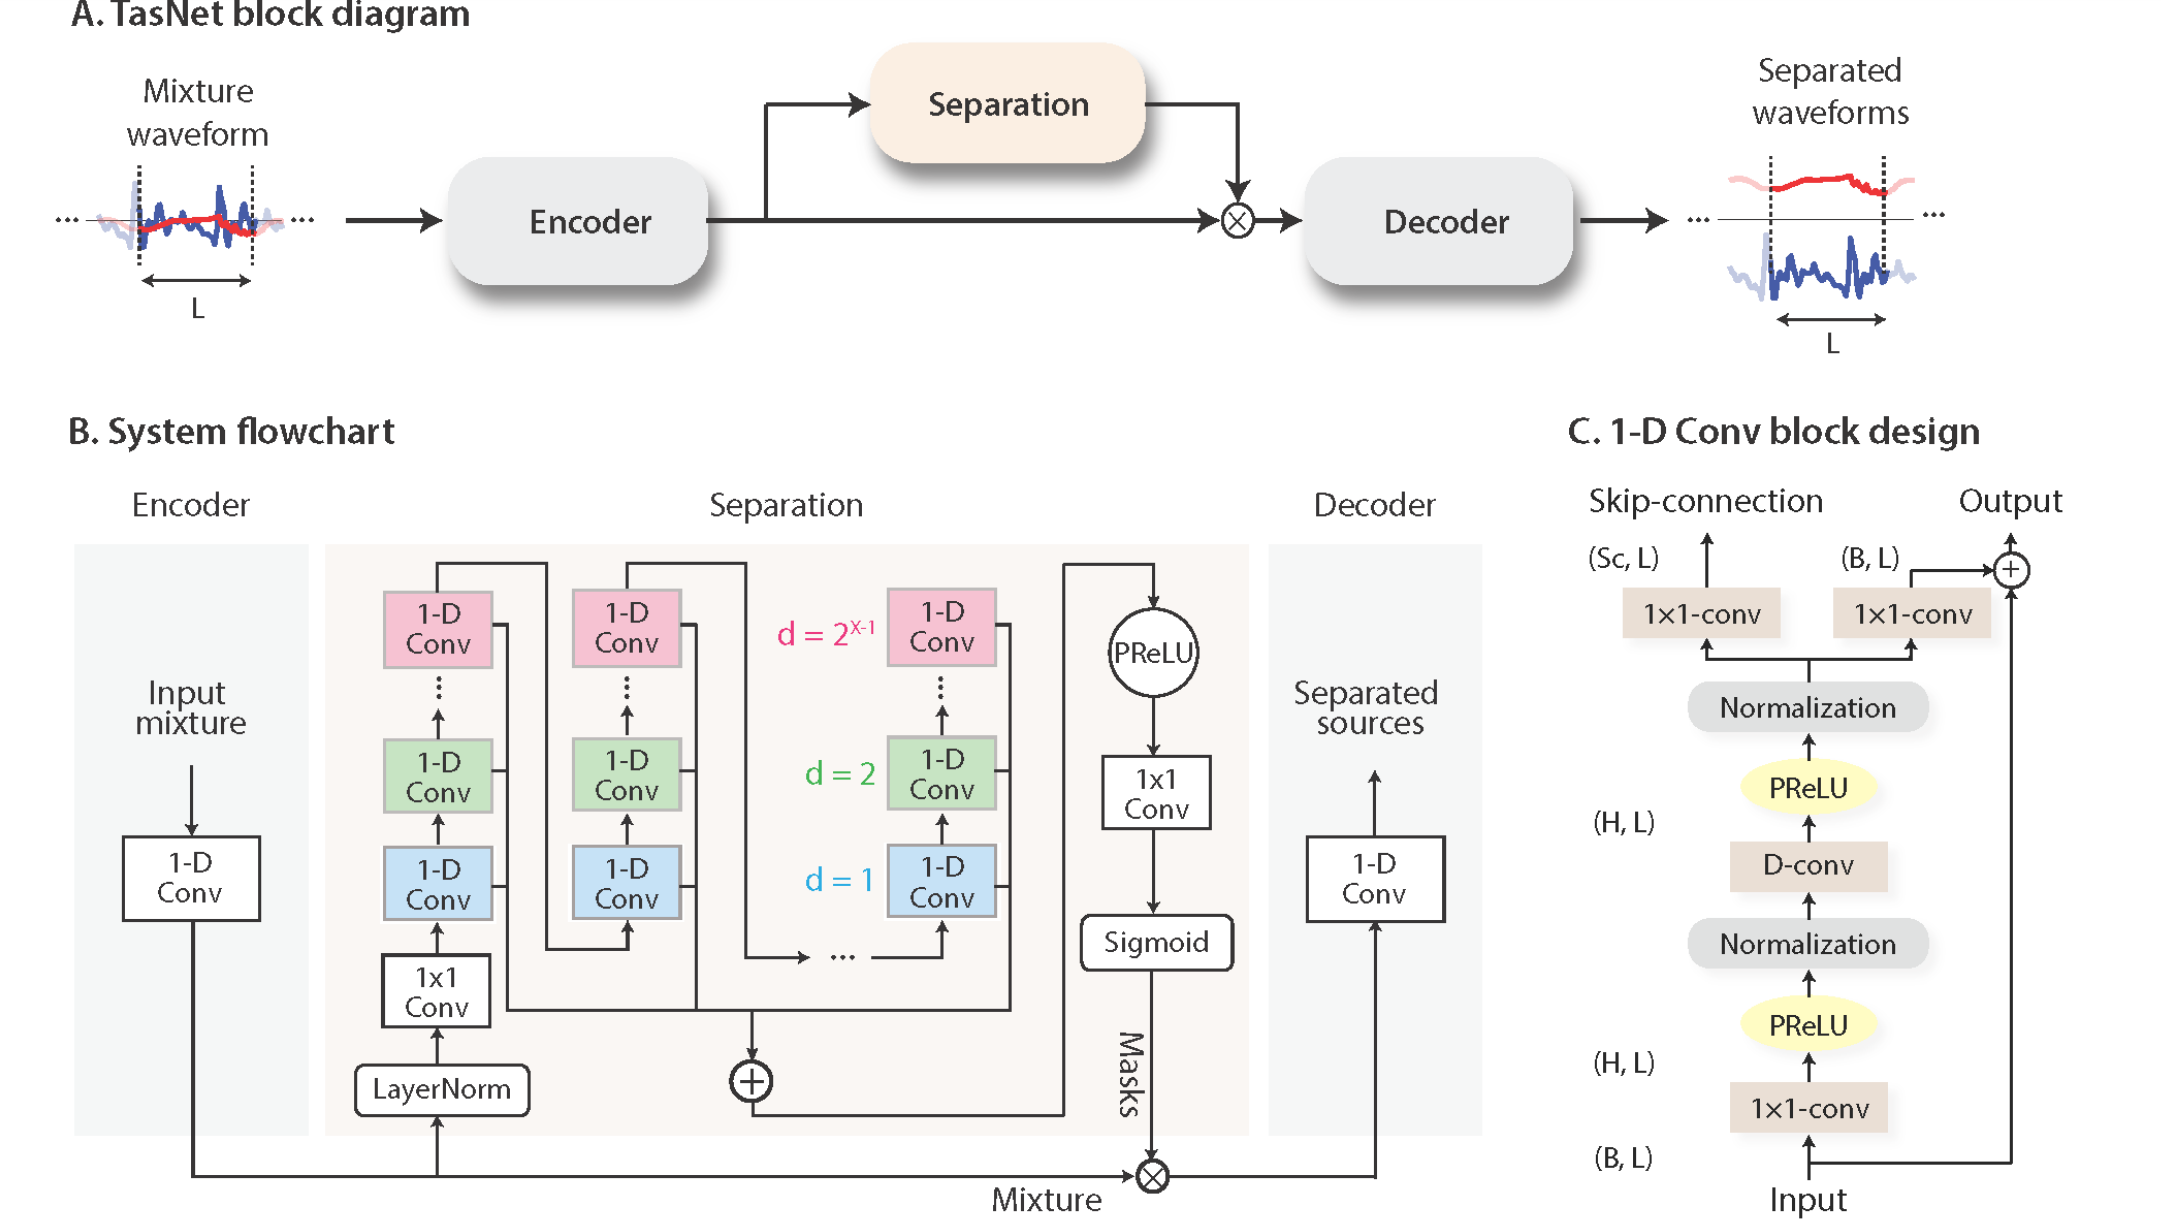
\includegraphics[width=\textwidth,keepaspectratio]{conv-tasnet.png}
    \caption{\label{fig:convtasnet}Conv-TasNet architecture overview \cite{Luo2018ConvTasNetSI}.}
\end{figure}

The encoded features are passed to a \gls{tcn}, which serves as the core separation module. The \gls{tcn} is composed of two stacks, each containing four residual blocks, for a total of eight layers. Each residual block consists of a dilated convolution with exponentially increasing dilation factors (e.g., 1, 2, 4, 8), followed by group normalisation (with eight groups), a \gls{prelu} activation, and a second projection convolution. A residual connection is used to stabilize training and preserve input information. The dilation strategy allows the \gls{tcn} to model long-range temporal dependencies efficiently while maintaining a fixed receptive field size.

Unlike the original \gls{convtasnet}, which applies explicit time-domain masking for source separation, this implementation omits masking altogether. Instead, the \gls{tcn} directly outputs an enhanced latent representation, which is then decoded into denoised real and imaginary spectrogram components via a final \(3 \times 3\) convolutional layer. This simplifies the architecture, as masking yielded marginal gains.

The output of the decoder is aligned with the original input size by cropping along both frequency and time axes to correct for minor size mismatches introduced by convolutional operations. This ensures a consistent dimensionality before inverse \gls{stft} reconstruction.

By preserving the temporal modelling strength of the original \gls{tcn} structure and adapting it to operate in the complex spectrogram domain, this implementation of \gls{convtasnet} offers a powerful yet flexible architecture for speech denoising. It combines deep receptive fields, efficient convolutional modelling, and skip connections within residual blocks to robustly recover clean speech across variable-length inputs.

\vspace{2em}

This project explores several neural network architectures for speech enhancement, starting with a simple \gls{cnn}-based autoencoder. It then advances to \gls{fcn} models like \gls{ced} and \gls{rced}\~\cite{park2017acoustic}, followed by \gls{unet} with skip connections and deeper encoding. Finally, \gls{convtasnet} ~\cite{Luo2018ConvTasNetSI}, originally designed for time-domain speech separation, is adapted for spectrogram-based denoising using its \gls{tcn}. These models provide a diverse framework, highlighting trade-offs in design and establishing strong baselines against classical techniques.

